
\chapter{The Results Manager}

The Results Manager, corresponding to the Results tab\index{Results tab} of the GUI, has
two main responsibilities: to manage simulation runs for this project
(Section~\ref{sec:managing-simulation-runs}) and to allow the
interrogation of these simulation runs through the use of
\emph{indicators}
(Section~\ref{sec:interrogating-results-with-indicators}). We explore
both of these in this chapter.

\section{Managing simulation runs}
\label{sec:managing-simulation-runs}

The ``Simulation runs'' node captures all
available simulation runs for this project. For example, when a
simulation is run from the ``Scenarios-manager'' (see
chapter~\ref{chap:scenarios-manager}), an entry is made under
``Simulation runs''. If for some reason a run that you know exists
for this project is not listed, right-click on 
``Simulation runs'' and select ``Import run from disk'' (See
Figure~\ref{fig:results-manager-import-run}). The GUI will try to load
the missing run and make it available.

\begin{figure}[htp]
\begin{center}
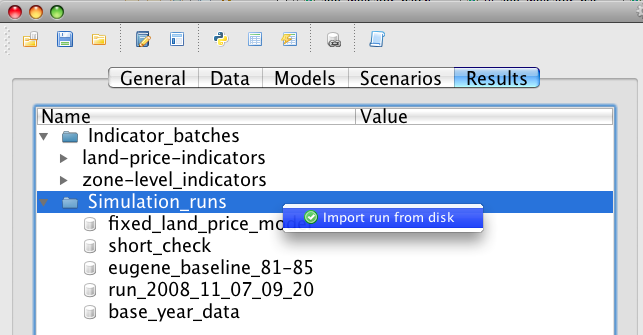
\includegraphics[width=.8\textwidth]{part-gui/images/result-manager-import-run-from-disk.png}
\end{center}
\caption{Importing a run from disk that is not showing up as a
``Simulation run''.}
\label{fig:results-manager-import-run}
\end{figure}

A couple operations can be performed on a simulation run. To view
information about a given run, right-click on the run and select
''Show details''. To remove all traces of a simulation run,
including the data on disk, right-click on the run and select
''Remove run and delete from harddrive''.

\section{Interrogating Results with Indicators}
\label{sec:interrogating-results-with-indicators}

Indicators are variables defined explicitly for use as a meaningful
measure (see Chapters~\ref{chap:variable-library} and 
\ref{chapter:expressions}). Like model variables,
they can be defined using the domain-specific programming language via
the ``Variable Library'' accessible through the Tools menu (see
Chapter~\ref{chap:variable-library}). An indicator can then be
visualized as either a map or as a table in a variety of
formats. The GUI provides two ways to use indicators to understand what
has happened in a simulation run: interactive result exploration
(Section~\ref{sec:interactive-result-exploration}) and Batch
indicator configuration and execution
(Section~\ref{sec:batch-indicator-configuration}).

\subsection{Interactive result exploration}
\label{sec:interactive-result-exploration}
Often, it is desirable to explore simulation results in a lightweight
fashion in order to get a basic idea of what happened. You don't
necessarily want to go through the process of exporting results to a
GIS mapping tool in order to gain some basic intuitions into spatial
patterns.

The Opus GUI's ``Result Browser'', available from the ``tools''
menu\index{Tools menu!Result Browser}, allows interactive exploration of simulation results. The Result
Browser presents a selectable list of available simulation runs, years
over which those simulations were run, and available indicators. You
can then configure an indicator visualization by selecting a simulation
run, a year, and an indicator. To compute and visualize the configured
indicator, simply press the ``generate results'' button (See
Figure~\ref{fig:results-manager-result-browser}). The
indicator will then be computed for the year of the selected simulation
run. After it is computed, a tab should appear at the bottom of the
window with the name of the indicator. Subtabs allow you to see the
results as a table or map (using the Matplotlib Python module). 

\begin{figure}[htp]
\begin{center}
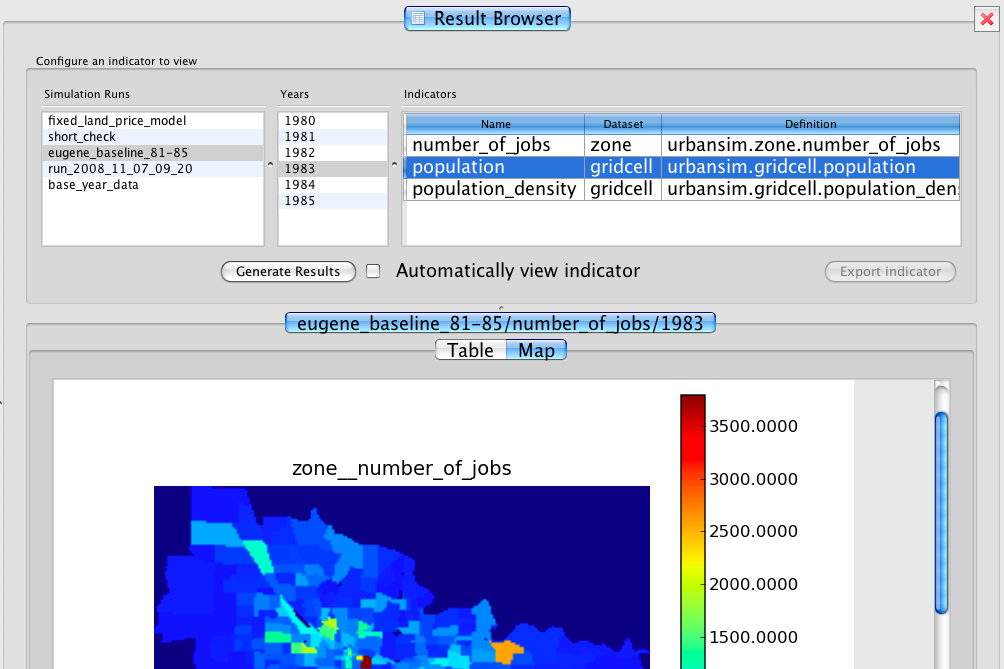
\includegraphics[width=1.0\textwidth]{part-gui/images/result-manager-result-browser.png}
\end{center}
\caption{Using the ``Result browser'' for interactive result
exploration.}
\label{fig:results-manager-result-browser}
\end{figure}

\fbox{
\begin{minipage}{.5\linewidth}
\begin{enumerate}
  \item Open the Results Browser from the Tools menu. Use the
  Results Browser to answer the following questions.
  \item Just from visual inspection, is there more than one cluster of
  gridcells with high land value in the Eugene region in 1980 in the
  baseyear data?
  \item Is this cluster(s) in the same general area as the
  greatest number of jobs in Eugene for the same year of the
  baseyear data?
\end{enumerate}
\end{minipage}
}

Two additional aspects of the Result Browser should be mentioned:
\begin{enumerate}
  \item If the checkbox ``Automatically view indicator''\index{Tools menu!Result Browser!view indicator automatically}\index{indicator!view indicator automatically} is
  clicked, everytime you change the indicator configuration (i.e.
  select a different simulation run, year, or indicator), the
  indicator will be automatically visualized (as if you pressed the
  ``Generate results'' button). 
  \item The ``Export results''\index{Tools menu!Result Browser! export results of indicator}\index{indicator!export results}button will export the table data
  of the currently configured indicator to a database. This feature
  is not yet implemented. 
\end{enumerate}

\subsection{Batch indicator configuration and execution}
\label{sec:batch-indicator-configuration}

The ``Result Browser'' is good for poking around in the
data. But often you'll want to generate the same
set of indicators for each of many runs and you don't want to
redefine them every time. Instead, you'd like to configure and save a
group of them that can be executed on demand on an arbitrary
simulation run. In the Opus GUI, this functionality is supported with
\emph{indicator batches}. 

To create a new indicator batch\index{indicator batch}, right-click on the
 ``Indicator\_batches'' node in the ``Results tab'' and select
 ``Add new indicator batch...'' (See
Figure~\ref{fig:results-manager-new-batch}). A new batch will be
created under the Indicator\_batches node.

\begin{figure}[htp]
\begin{center}
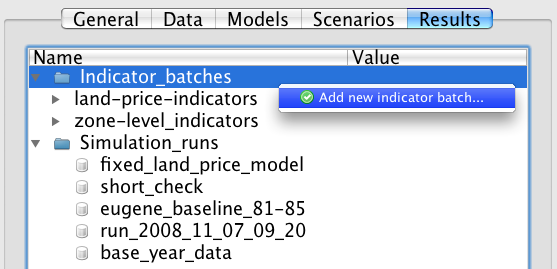
\includegraphics[width=.6\textwidth]{part-gui/images/result-manager-add-new-batch.png}
\end{center}
\caption{Creating a new indicator batch}
\label{fig:results-manager-new-batch}
\end{figure}

A batch is a collection of ``Indicator visualization''
definitions. Each indicator visualization\index{indicator visualizations} is a configuration of
the indicator variable to be used, a visualization style (e.g. map or
table), and some format options. To add a new indicator visualization
to the batch, right-click on the respective batch and select
``Add new indicator visualization...''\index{indicator visualizations!adding an indicator visualization}. A dialog box will
appear where you can define the visualization. The visualization
options for an indicator visualzation are discussed in depth later.

You can add as many indicator visualizations to a batch as you want. In
order to execute an indicator batch on a simulation run, right-click on
the indicator batch and hover over
 ``Run indicator batch on...''\index{indicator visualizations!running an indicator batch}. A list of all the available simulations
 runs will
appear as a submenu. You can then select the appropriate simulation.
The indicator visualizations in the batch will be executed over all the
years of that simulation run. If the resulting indicators are tables or
maps stored in a file, they can then be found on disk in your
``OPUSHOME/data/PROJECTNAME/runs/RUNNAME/indicators'' directory, where
``PROJECTNAME'' is the name of your project (e.g.
 ``eugene\_gridcell'') and ``RUNNAME'' is the name of the
simulation run that you selected to run the batch on. The indicator
visualizations configured to write to a database will have produced
tables in the specified database with the name of the respective
indicator visualization.

\fbox{
\begin{minipage}{.5\linewidth}
Create, configure, and execute a new indicator batch:
\begin{enumerate}
\item Create a
new indicator batch by right-clicking on the  ``Indicator\_batches'' node
in the Results tab\index{Results tab!indicator batch} and selecting the appropriate option. 
\item Add an indicator visualization configuration to
that batch. Right-click on your new indicator batch and select  ``Add new
indicator visualization''.
\item Configure a Map visualization that contains the 
{\sf zone\_job\_density} and {\sf zone\_population\_density} indicators for the
zone dataset.
\item Close the batch visualization configure dialog.
\item Right-click on the batch and
execute your indicator batch on the results of a simulation run.
\end{enumerate}
\end{minipage}
}


\subsubsection{Indicator visualization configuration options}
\label{sect:indicator-visualization-options}

Opus provides a variety of ways to visualize indicators\index{indicator visualizations!configuration} and this
functionality is exposed in the ``Indicator visualization'' dialog
box options (e.g. multi-year indicators, exporting to
databases). This section describes the range
of available options in the Batch indicator visualization dialog
box, which is separated into three components:  ``indicator
selection'',  ``output options'', and  ``format options'' (See
Figure~\ref{fig:results-manager-batch-viz}). 

\begin{figure}[tph]
\begin{center}
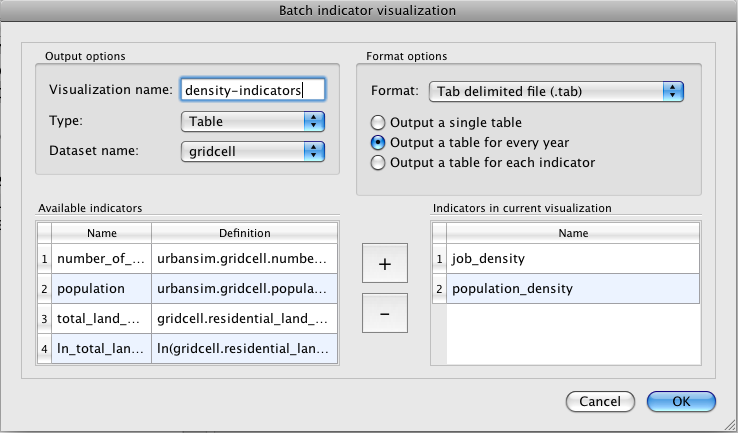
\includegraphics[width=\textwidth]{part-gui/images/result-manager-batch-viz-config.png}
\end{center}
\caption{The batch visualization creation dialog.}
\label{fig:results-manager-batch-viz}
\end{figure}

\heading{Indicator selection}

The bottom of the dialog box has two list boxes,  ``available
indicators'' and  ``indicators in current visualization''. The
indicators here are those variables defined in the 
``Variable Library'' (Chapter~\ref{chap:variable-library}) whose
\emph{use} has been set to be \emph{indicator} or \emph{both}. Note that the set of
indicators available is filtered by the currently selected dataset in
the  ``output options'' (described later in this section).

By moving an indicator from the  ``available indicators''\index{indicator!available indicators} box to the
 ``indicators in current visualization'' bo\index{indicator!indicators in current visualization} via the  ``+'' button, you
include that indicator in this indicator visualization. Likewise, to
remove an indicator from the visualization, select the indicator in
the  ``indicators in current visualization'' box and press the  ``-''
button.


\heading{Output options}

\emph{Visualization Name}. The base name of any produced
visualizations\index{indicator visualizations!visualization name}. Because you might be producing this visualization for
different years and different simulation data, more information will
be appended to this name to ensure uniqueness of the resulting file
or database table when the visualization is run on some data. 

\emph{Type}. There are two different types of indicator
visualizations\index{indicator visualizations!visualization types} that can be produced: maps and tables. Tables are just
raw data organized into rows and columns, while maps are
spatial projections of this data. The available format options
(described later) are fully dependent on the visualization type. 

\emph{Dataset name}. The dataset that this visualization\index{indicator visualizations!dataset} corresponds
to. When the selected indicator(s) are run, they will be computed over
this dataset. Most commonly you are choosing a geographic granularity
(e.g. gridcell, zone) that you want to see the results at. Note that
when you change the dataset, the set of available indicators changes
because a given indicator is valid only for a single dataset.

\heading{Format options for maps}

Map visualizations\index{indicator visualizations!visualization types!map format options}  will produce a map file for every selected
indicator for every available year when it is executed on a
simulation run. 

The available map format is Mapnik, a free toolkit for developing 
mapping applications (http://mapnik.org/).  Note that the Mapnik maps 
are not intended to replace GIS-based mapping, which allows far more 
control and the overlay of other features for visual reference. It 
is merely a quick tool to visualize data to get a sense of the 
spatial patterns in it.  In order to support visualization in a 
GIS environment such as ArcGIS or QGIS, the results may be exported 
to a database or geodatabase environment, and the GIS software used 
to create a more interactive and flexible display of the data. See 
the following section for a description of how to export indicator 
results to a SQL database or a DBF file for use in external GIS tools.

\fbox{
\begin{minipage}{.5\linewidth}
Export the results that were found in the previous tutorial inset
to a SQL database. 
\begin{enumerate}
  \item Make sure that you have configured a database
server. From the Tools menu, select  ``Database Server Connections''\index{Database Server Connections}. Check
to see that the ``indicators\_database\_server" is correctly set up.
If you don't have a remote database server, make sure that it
points to a sqlite connection. Close the
connections dialog box.
  \item Reconfigure the batch to write to a
database. Expand the indicator batch that you defined in the prior
step. Right-click on the visualization and select ``Configure
visualization''. Change the format to ``Export to SQL database'' and then
name a database it should write to. Hit OK and then rerun the batch on the
simulation results from before.
  \item Launch a database browser and check to see if the proper
  tables were created. 
\end{enumerate}
\end{minipage}
}

To set the Mapnik map options, in the batch visualization creation 
dialog window (shown above) select "Map" from the "Type:" drop-down menu, 
then click the "Mapnik Map Options" button that will appear directly below the 
"Format:" drop-down menu. In the Mapnik Map Options dialog window, all 
of the mapping options can be set.

\begin{figure}[h]
\begin{center}
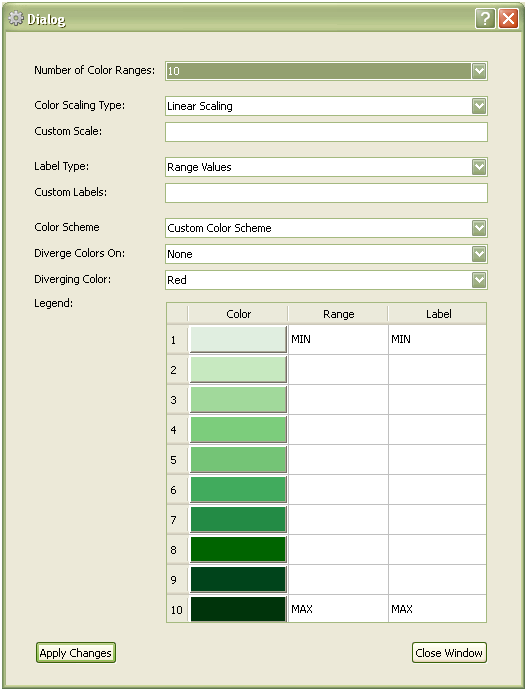
\includegraphics[width=3in]{part-gui/images/result-manager-mapnik-options-dialog.png}
\end{center}
\caption{The map options dialog window showing default settings.}
\label{fig:result-manager-mapnik-options-dialog}
\end{figure}

\emph{Number of Color Ranges}. This sets the number of 
buckets to split the range of the values 
being mapped in to. The drop-down menu allows you to choose a 
number between 1 and 10.

\emph{Color Scaling Type}. This drop-down menu 
allows you to choose between "Linear Scaling" 
and "Custom Scaling". Linear scaling will evenly divide of the 
range of values to be mapped into buckets of the same size.  
Custom scaling will let you specify how to divide the range of values 
into the buckets. 

\emph{Custom Scale}. If "Custom Scaling" is selected 
as the Color Scaling Type, then 
the values in this text field will be used to define the bucket 
ranges. For example, if the following string is entered in 
the Custom Scale text field "5, 100, 2000, 40000", then the bucket 
ranges will be '5 to 100', '100 to 2000', and '2000 to 40000'.  
Also, if either "min", "MIN", "max", or "MAX" is entered in the 
Custom Scale text field, they will be replaced with the minimum 
or maximum values of the values that are being mapped. For example, 
"min,100,max" is a valid entry for Custom Scale.

\emph{Label Type}. This drop-down menu allows 
you to choose between "Range Values" and 
"Custom Labels" to use as the labels on the color bar that will 
be drawn in to the map image. Using range values means that the 
boxes in the color bar will be labeled with the range of values that 
are being colored with the color contained in the corresponding box. 
Using custom labels allows you to manually enter the labels 
for each box.

\emph{Custom Labels:}. If "Custom Labels" is 
selected as the Label Type, then the values 
in this text field will be used to label the colored boxes in the 
color bar. For example, if the following string is entered in 
the Custom Labels text field "a,b,c,", then the first box will 
be labeled "a", the second will be labeled "b", and the third 
will be labeled "c".

\emph{Color Scheme}. This drop-down menu allows you to choose between "Custom Color Scheme", 
"Green", "Blue", "Red", and "Custom Graduated Colors". The color 
buttons in the legend are buttons, that when pushed, cause a color 
chooser dialog window to pop up that can be used to pick the color of 
the box. If Custom Color Scheme is selected, then all manually-set colors 
will be saved when the "Apply Changes" button is pushed, whereas all colors 
will be over-written when the "Apply Changes" button is clicked if any other 
color scheme option is selected. If Green, Blue, or Red is selected, the 
boxes will be colored with pre-defined colors. Lastly, if Custom Graduated 
Colors is selected, then the boxes will be colored in an even, graduated 
scale where the range of colors starts at the current color of the box at 
index 1 and ends at the current color of the box at the highest index.

\emph{Diverge Colors On}. This gives you the option to 
have two diverging colors. You have to option 
"None" to split on none of the indices to use just one color scale, or 
you have the option to split on any index from 1 to 10. The box at the 
selected index will be set to white and the two color scales above and 
below it will be set based on what color option is selected in the Color 
Scheme and Diverging Color drop-down menus. Note that if "Custom Graduated Colors" 
is selected in the Color Scheme drop-down menu, then the two color 
scales above and below the box at the diverging index will have graduated 
color scales and the option selected in the Diverging Color drop-down menu 
will be ignored.

\emph{Diverging Color}. This drop-down menu allows 
you to choose between "Red", "Green", and "Blue".  
This will set the color for the boxes with an index number lower than 
the index number selected in the Diverge Colors On drop-down menu.

\clearpage
\heading{Examples of how to create default and custom maps}

\emph{Create a default map}. To create a map with the default settings 
(using the Eugene gridcell project), create an indicator batch and 
in the batch indicator visualization dialog window, , set Type to 
"Map", set Dataset name to "zone", and select "number_of_jobs" to be 
included in the current visualization.  Then run the indicator batch on 
a simulation. This will produce a map with the default 
settings of 10 color ranges, colored green, where each color range is 
the same size and linearly increasing from light green to dark green.
For instructions on how to create and run an indicator batch see section
\ref{sec:batch-indicator-configuration}. The map will look like the 
map shown below.

\begin{figure}[ht]
\begin{center}
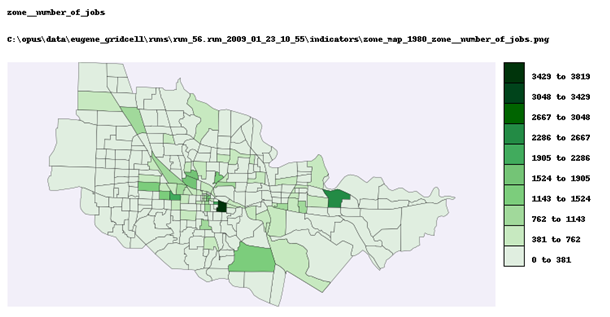
\includegraphics[width=\textwidth]{part-gui/images/sample-map-default-settings.png}
\end{center}
\caption{A Mapnik map colored with the default color scheme.}
\label{fig:sample-map-default-settings}
\end{figure}
\clearpage

\emph{Create a custom map}. To create a customized map, 
open the batch indicator visualization window (see section 
\ref{sec:batch-indicator-configuration} for information on 
how to do this), for the map created in the \emph{Create a default map}
section and click on the Mapnik Map Options button that is directly 
below the Format drop-down menu.

Suppose that we would like to create the same map again, but this time 
with 9 color ranges, custom ranges, custom labels, and a diverging color 
scheme where all values from 0 to 300 are colored with gradually lighter 
shades of blue and all values from 300 to 4000 are colored with gradually 
darker shades of red. As a side note, the option to use a diverging color 
scheme exists primarily to allow the coloring scheme to differentiate 
between positive and negative values.  However, all values in 
this example are all greater than or equal to zero.

Select "9" in the Number of Color Ranges drop-down menu, select 
"Custom Scaling" in the Color Scaling Type menu, enter 
"0,50,100,150,200,300,400,500,1000,4000" in the Custom Scale text field, 
select "Custom Labels" in the Label Type menu, enter "a,b,c,d,e,f,g,h,i" 
in the Custom Labels text field, select"Red" in the Color Scheme menu, 
select "6" in the Diverge Colors On menu, select "Blue" in the Diverging 
Color menu, and the press the Apply Changes button.

The color box at the index specified in the Diverge Colors On menu 
will be set to white. This color can be changed to a light pink 
color by clicking on the box to bring up a dialog window that lets 
you choose a new color. From the color chooser dialog window, select 
a light pink color and press OK.  Change the selected option in the 
Color Scheme menu to "Custom Color Scheme" so that your custom color 
for the box at index 6 will be saved when the Apply Changes button 
is pressed, and then press the Apply Changes button. The mapnik 
options dialog window should look like the screenshot pictured below. 
The map that will be created after the indicator batch has been run 
is also shown below. (see section \ref{sec:batch-indicator-configuration}
for information on how to run an indicator batch)

\begin{figure}[hb]
\begin{center}
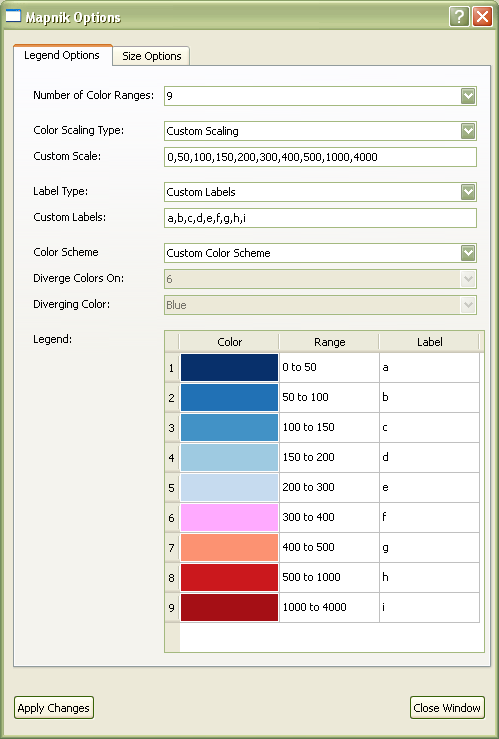
\includegraphics[width=3in]{part-gui/images/result-manager-custom-mapnik-settings.png}
\end{center}
\caption{The Mapnik map options window showing custom settings.}
\label{fig:result-manager-custom-mapnik-settings}
\end{figure}
\clearpage

\begin{figure}[hbp]
\begin{center}
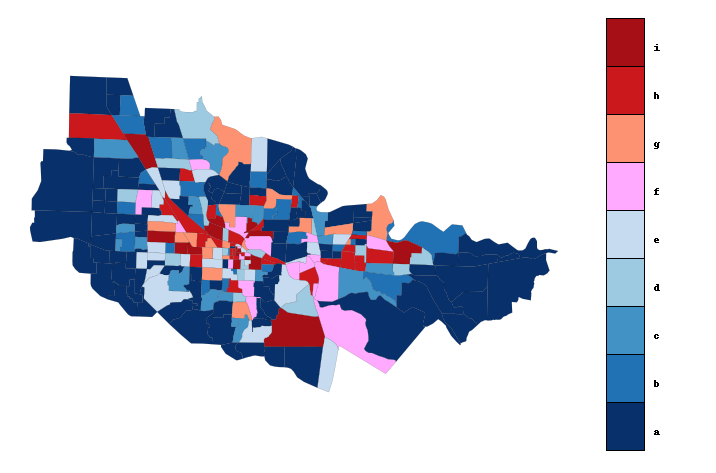
\includegraphics[width=\textwidth]{part-gui/images/sample-map-custom-settings.png}
\end{center}
\caption{A Mapnik map with a custom color scheme.}
\label{fig:sample-map-custom-settings}
\end{figure}
\clearpage

\emph{Create a custom graduated color scheme}. 
To create a map with a custom graduated color scale, 
re-open the Mapnik Options dialog window for the map 
created in the \emph{Create a custom map} section and select 
"Custom Graduated Colors" from the Color Scheme menu.  Click 
on the box in row 1 and select a light shade yellow, click on 
the box in row 9 and select a bright shade of blue, and click 
Apply Changes. The colors in boxes 2 through 8 will then be automatically set 
to create a graduated color scheme that spans from light 
yellow to bright blue. The mapnik options window and resulting 
map are shown below.

\begin{figure}[htp]
\begin{center}
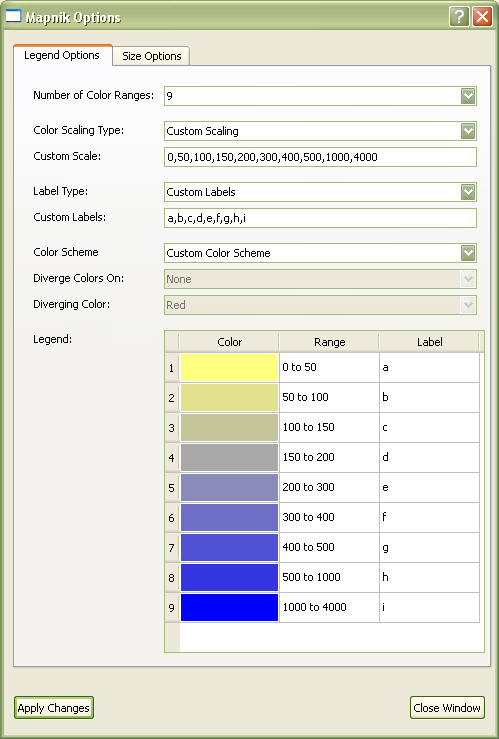
\includegraphics[width=3in]{part-gui/images/result-manager-mapnik-options-example-2.png}
\end{center}
\caption{The Mapnik map options window showing a custom graduated color scheme.}
\label{fig:result-manager-mapnik-options-example-2}
\end{figure}

\begin{figure}[hbp]
\begin{center}
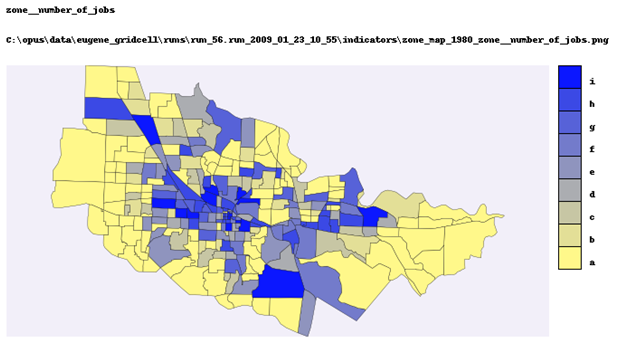
\includegraphics[width=\textwidth]{part-gui/images/sample-map-custom-settings-2.png}
\end{center}
\caption{A Mapnik map with a custom graduated color scheme.}
\label{fig:sample-map-custom-settings-2}
\end{figure}
\clearpage

\emph{Create a diverging custom graduated color scheme}. The graduated color 
schemes can also diverge on an index. Shown below is the Mapnik options 
dialog window with the same settings as set in the 
\emph{Create a custom graduated color scheme} section, 
but the selected option in the Diverge Colors On has been changed 
from "None" to "5".

\begin{figure}[hb]
\begin{center}
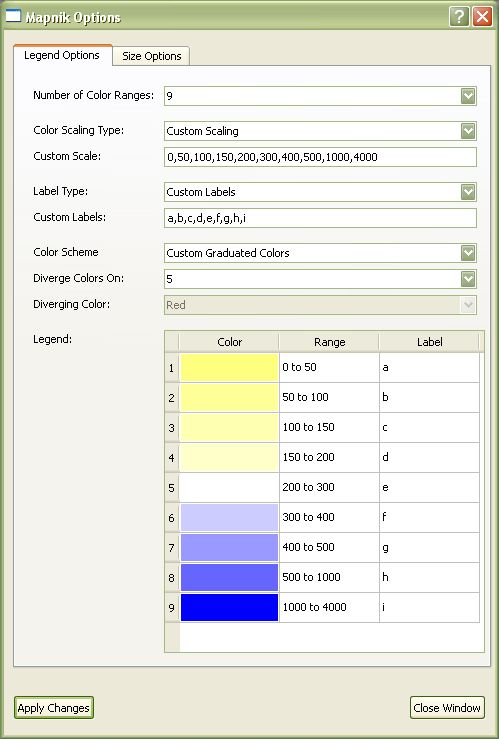
\includegraphics[width=3in]{part-gui/images/result-manager-mapnik-options-example-3.png}
\end{center}
\caption{The Mapnik map options window showing a diverging custom graduated color scheme.}
\label{fig:result-manager-mapnik-options-example-3}
\end{figure}
\clearpage

\heading{Format options for tables}

There are four different available formats for tables\index{indicator visualizations!visualization types!table format options}. Each has its
own parameters that need to be set. Note that the id column for the
dataset will automatically be included in all outputted tables
regardless of format.

\emph{Tab-delimited (.tab)}. This will output a file (or multiple
files) where the values are separated by tabs. There are three
different modes to choose from that affects how data is split across
files when the visualization is executed on a simulation run.
``Output in a single file'' will create single tab file that has a
column for each selected indicator for each year of the simulation
run. ``Output in a table for every year'' will create a tab file
for each year of the simulation run, with each column
corresponding to a selected indicator. Finally, 
``Output a table for each indicator'' will create a tab file for
each selected indicator, where each column
corresponds to the indicator values of a year of the
simulation run.

\emph{Fixed-field}. The fixed field format will output a single file
whose fields are written with fixed width and no delimiters. The file
contains a column for each selected indicator for each year of the
simulation run for which the visualization is being created. Format
info for each column needs to be specified. To specify the format of
the dataset id column, fill in the ``id\_col'' input field. To
specify the format of each selected indicator, enter the format in the
respective row of the ``field format'' column in the  ``indicators in
current visualization'' box. The field format has two parts, the length
of the field and the type. Available types are float ( ``f'') and
integer ( ``i''). Specified field formats follow the pattern  ``10i'' and
 ``5.2f'', where the latter specifies a float with five leading digits
with floating point precision carried out to two decimal places.

\emph{SQL database}. This format option can be used to export to an
arbitrary SQL database. The database server used is that specified in
the ``Database server connections'' under  ``indicators\_database''
(see Section~\ref{sec:database-server-connections}). The exported data
will take the form of a newly created in the specified database (if the database doesn't exist, it will be created
first). The SQL table will contain a column for every selected
indicator for every year of the simulation run that it is being
executed against. The name of the table is a combination of the name of
the visualization and the name of the simulation run. Additionally,
if you are exporting to a PostGRES database and have an existing
spatial table corresponding to the dataset of the visualization, a view
defining a join over the spatial table and the indicator table will
automatically be created. This allows you to instantly view the
indicator results in QGIS. 

\emph{ESRI database}. This option exports the
indicator data to an ESRI database that can be loaded into ArcMap.
Simply specify the path to a geodatabase file (.gdb). It is assumed 
that the geodatabase contains a \verb#Feature Class# corresponding to
the dataset of the indicator being exported. Once the export is
successfully completed, the geodatabase will contain a table that 
contains the indicator result, with a zone\_id and an
ArcGIS \verb#OBJECTID*# that corresponds to the internal object ids in
the feature class. It is safe to join the indicator table result with
the feature class using either the objectid or the zone\_id. See
Figure~\ref{fig:indicator-population-zone-arcgis} for an example
exported indicator after following this process. 

\begin{figure}[htp]
\begin{center}
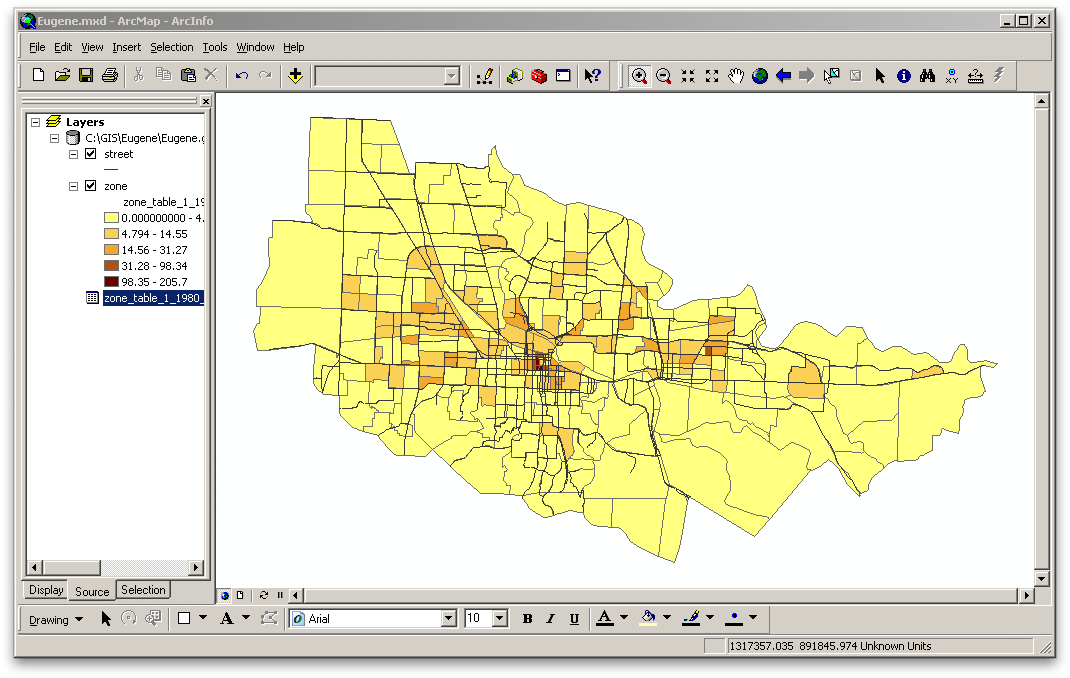
\includegraphics[width=.8\textwidth]{part-gui/images/result-manager-indicator-population-zone-arcgis.png}
\end{center}
\caption{Mapping a Population by Zone Indicator in ESRI ArcMap. Shows the result of
joining the feature class with the indicator table and generating a thematic map of the populaion by zone, using the zone.acres field to
normalize the population, resulting in a map of population density per
acre.}
\label{fig:indicator-population-zone-arcgis}
\end{figure}


